\section{Kode og Flowcharts}
	\subsection{Flowcharts}
		\begin{figure}[!h]
			\centering
			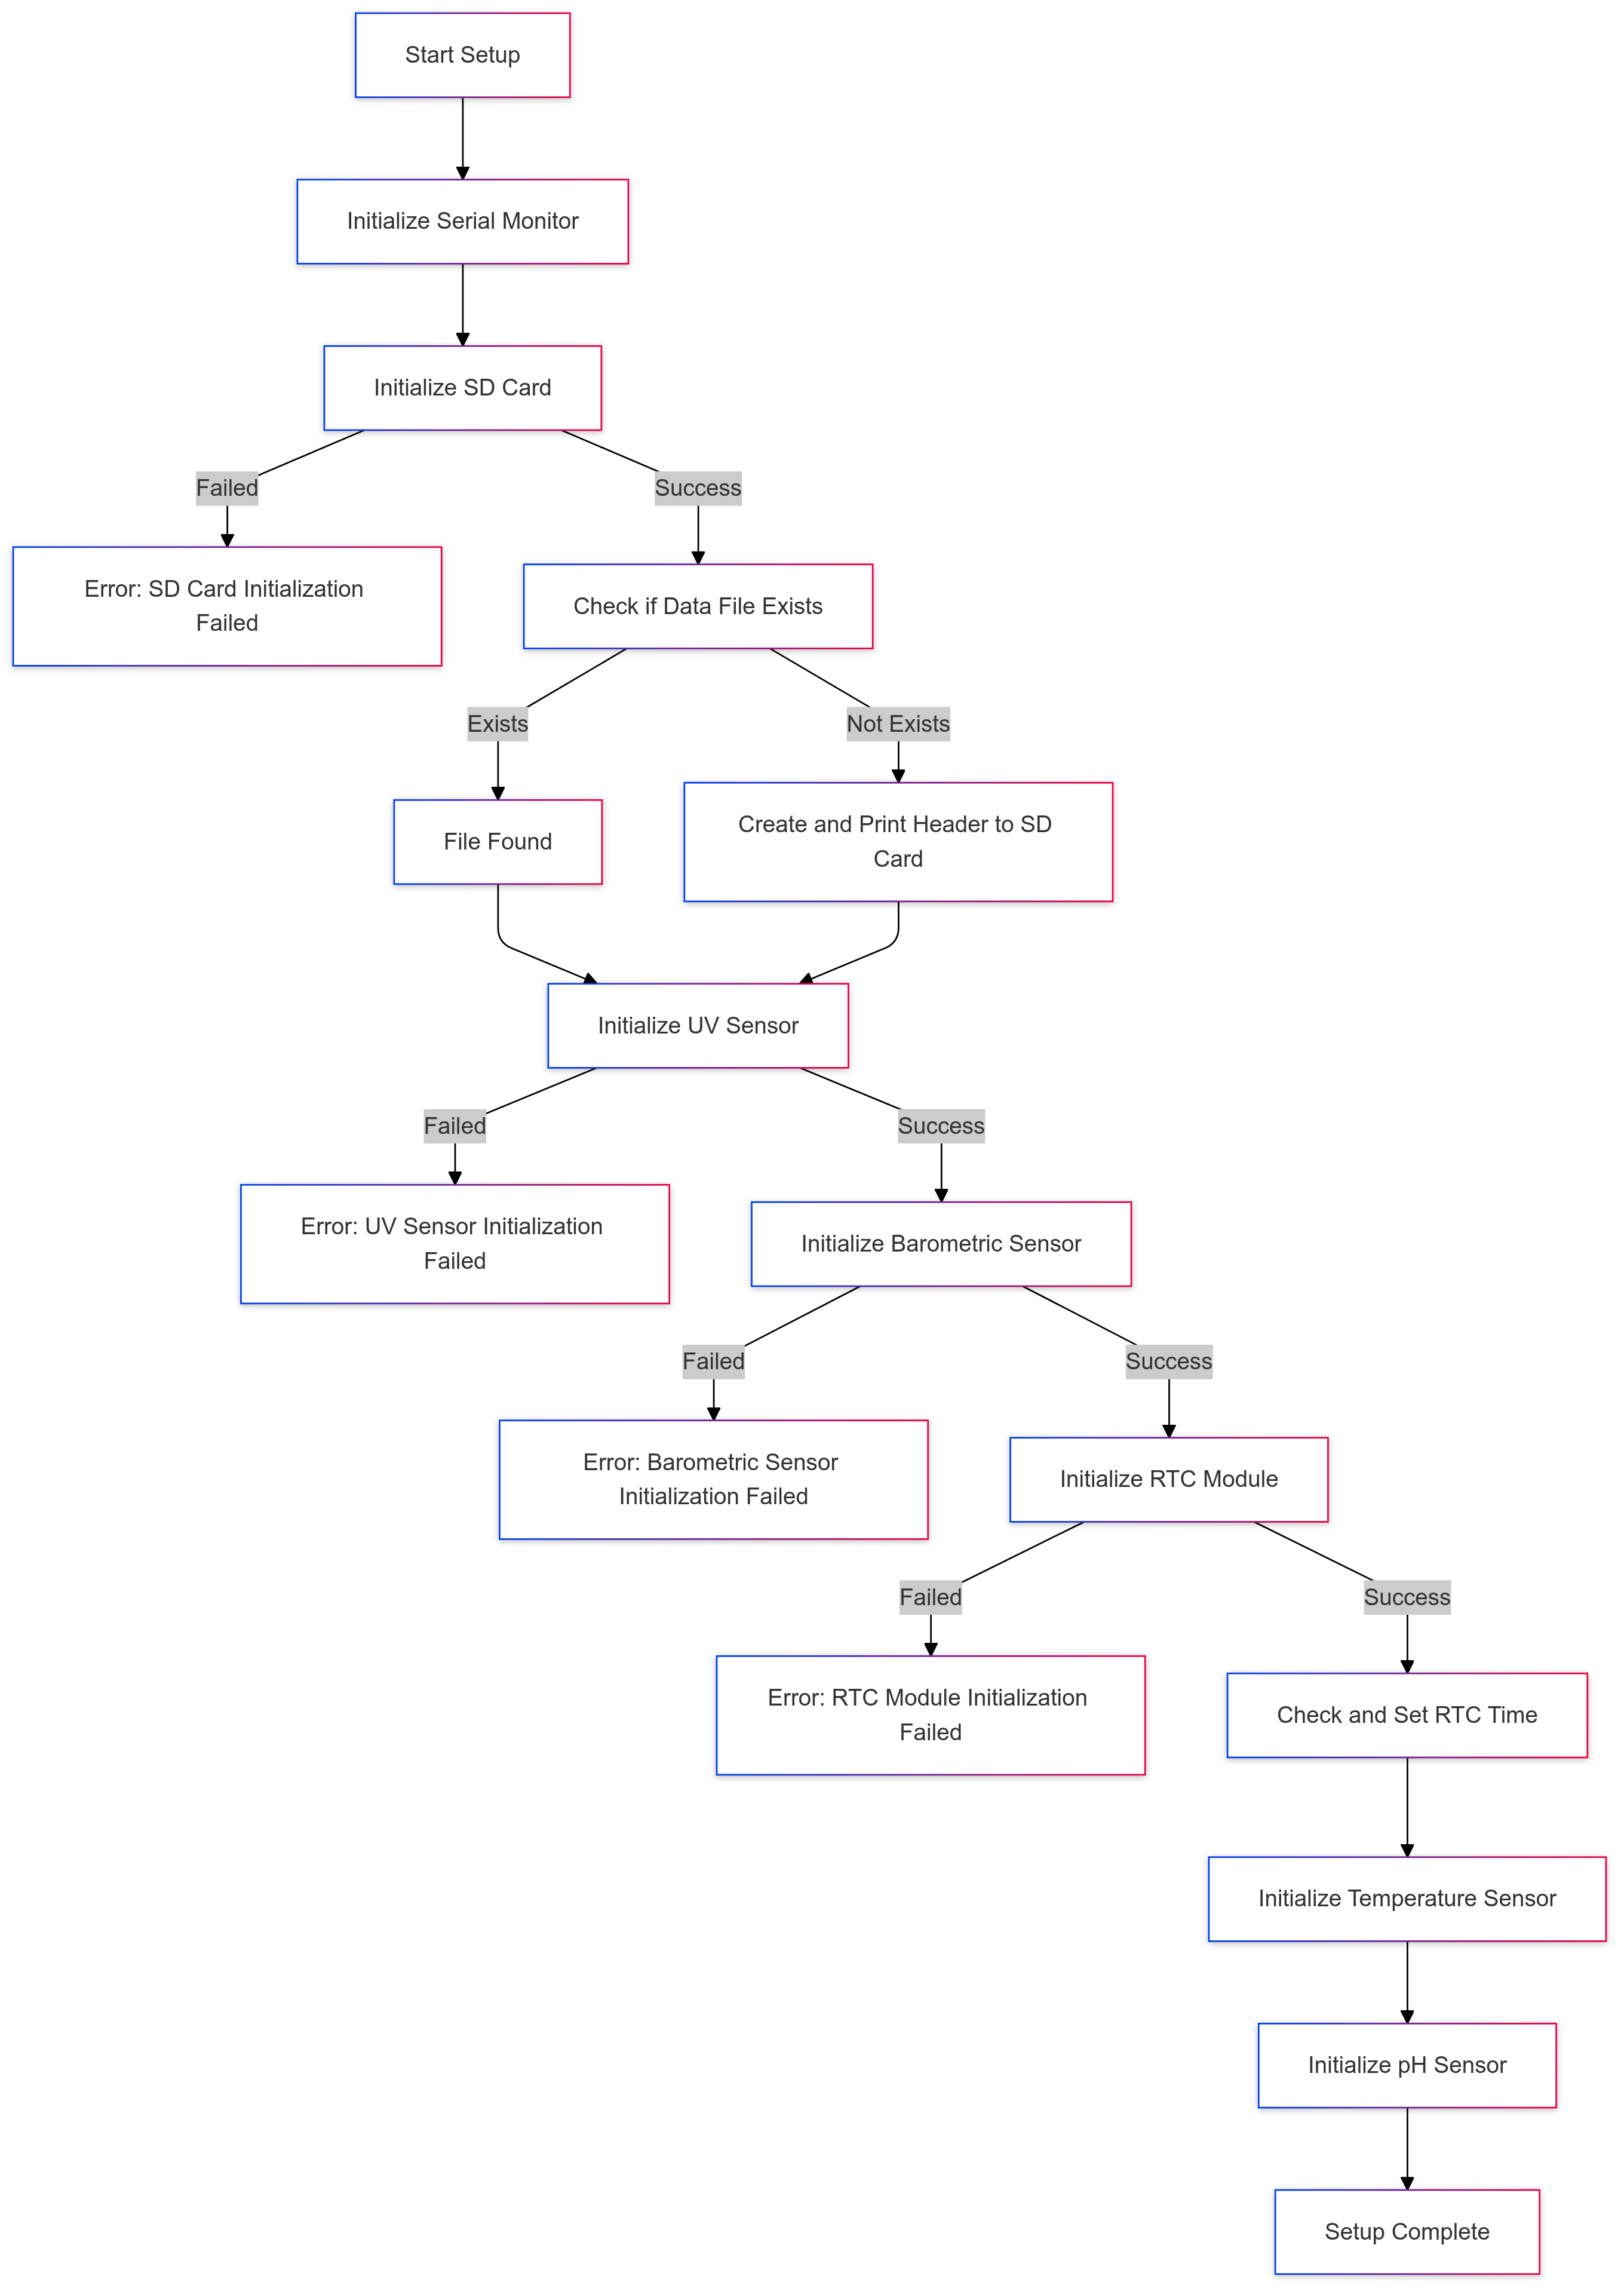
\includegraphics[width=0.9\textwidth]{Figures/Flowchart setup.png}
			\caption{Flowchart til setup funktionen}
		\end{figure}
		
		\begin{figure}[!h]
			\centering
			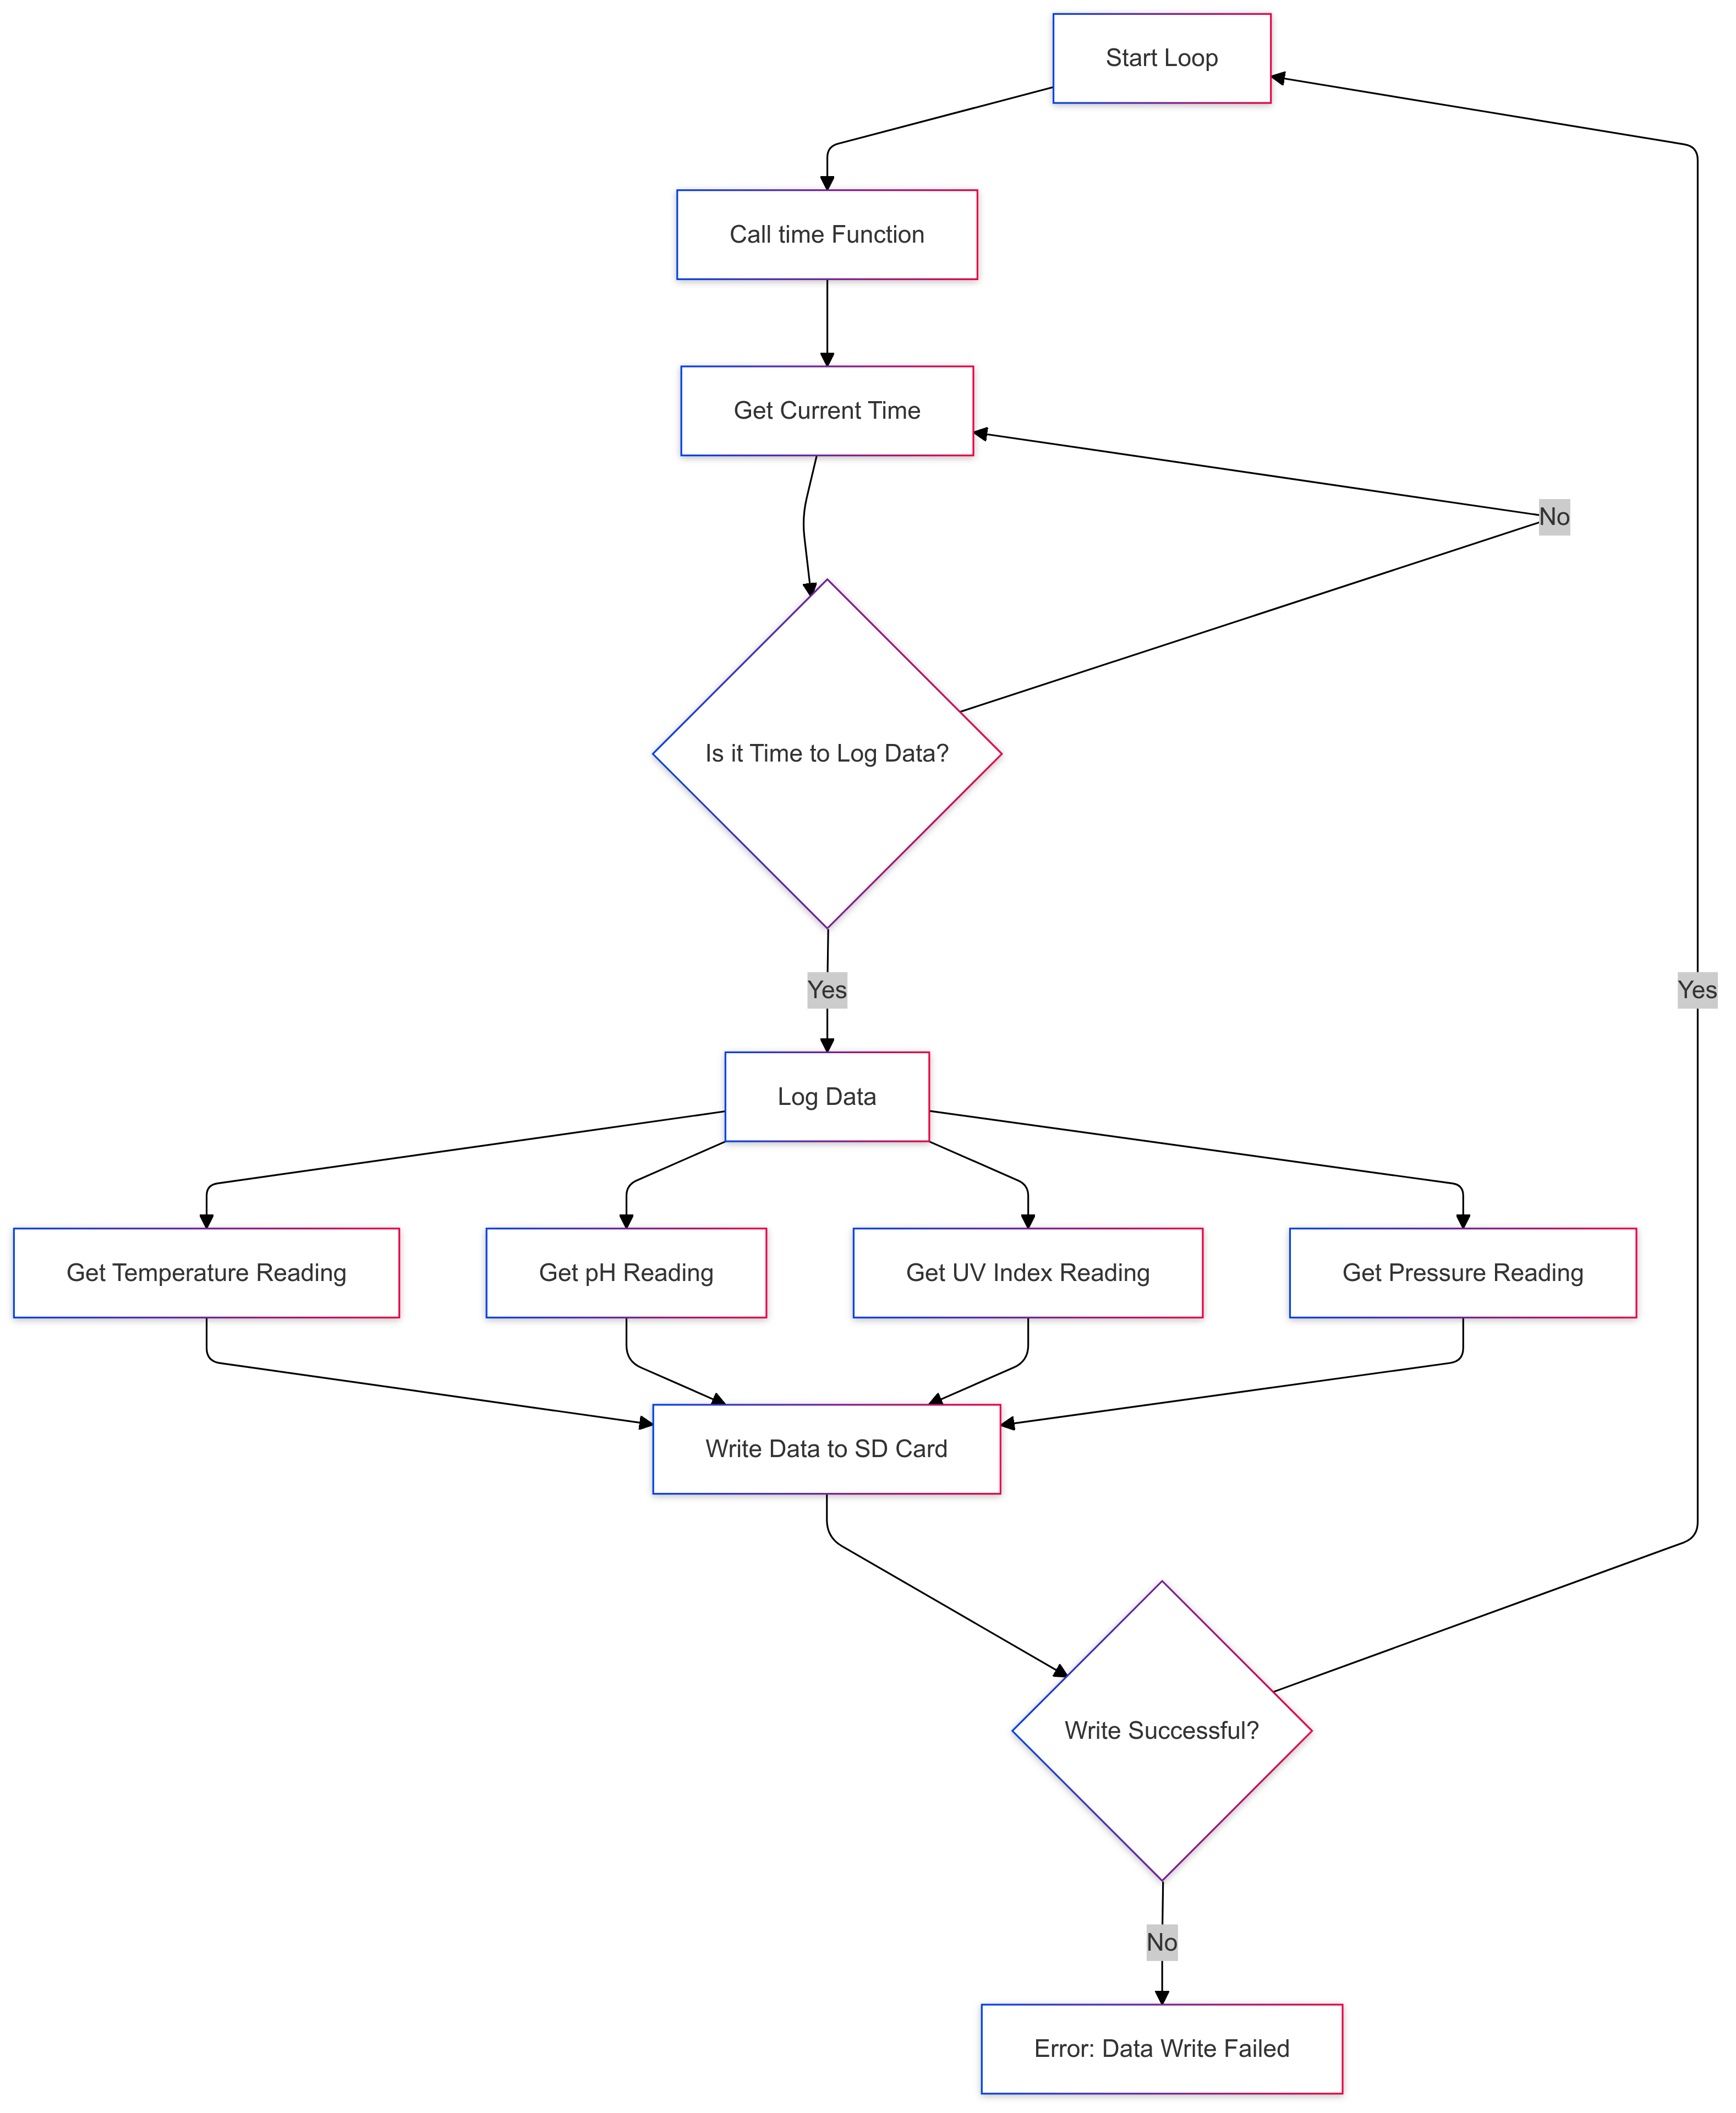
\includegraphics[width=\textwidth]{Figures/Flowchart loop.png}
			\caption{Flowchart til loop funktionen}
		\end{figure}
		
	\clearpage
	\newpage
	\subsection{Kode beskrivelse}
		Til koden er der importeret 9 biblioteker, hvor 7 af dem er til direkte brug af alle modulerne forbundet til Arduinoen.\\ [7pt]
		% Test koden uden de 2 sidste biblioteker
		Lige før setup funktionen bliver der defineret nogle globale variabler. Disse variabler er numrene på de pins, hvor modulerne er forbundet, navn på data filen som skal skrives til, tidsintervallet mellem måling af data, og nogle instanser, som giver nogle funktioner man kan bruge til at kommunikere med modulerne og sensorerne. En instans giver den defineret variabel nogle funktioner, som kan bruges. Det er funktioner, som bliver brugt ofte, og derfor er det lavet til noget, som kan kopires let. Eksempelvis er der i biblioteket, der hedder "Adafruit\_VEML6075.h"{} defineret en klasse, som hedder "Adafruit\_VEML6075"{}. Denne klasse har nogle funktioner i sig, og når man laver en instans af dette, hvilket f.eks. er gjort med variablen "uv"{}, så kan man tilgå alle klassens funktioner via variablen.
		\begin{lstlisting}
Adafruit_VEML6075 uv = Adafruit_VEML6075();
		\end{lstlisting}
		\vspace{15pt}
		Setup funktionen er en funktion, som kun bliver kørt én gang, når man starter Arduinoen eller genstarter koden. I setup funktionen sendes beskeder til alle modulerne som bruges, så de starter op og kan bruges. Et eksempel er, hvor der bliver kaldt "uv.begin()". Som forklaret ovenover, er uv en instans af en klasse med mange funktioner i, og .begin() er en af funktionerne, som kan bruges.\\ [5pt]
		I setup bliver der tjekket om der allerede findes en fil ved det navn, der er defineret. Man kan vælge at slette filen, hvis man gerne vil det. Det er der dog ikke behov for ved denne datalogger. Der bliver tjekket, om der findes en fil ved det defineret navn, fordi der skal tilføje en header linje til data filen, hvis det er tilfældet. Hvis Arduinoen startes op, og der allerede findes en fil ved det defineret navn, betyder det, at der allerede er data i filen. Derfor tilføjes der ikke en header linje. Hvis der ikke allerede er en fil ved det defineret navn, oprettes der en fil, og tilføjes en header linje, hvilket er navnene på dataet i hver kolonne, for at forklare, hvad de forskellige kolonners data er.
		\begin{lstlisting}
void header() {
	int attempts = 0;
	while (!writeToSDCard("Date, Time, Temperature, pH Value, UV Index, Pressure (hPa)\n")) {
		attempts++;
		// If the function could not print to the SD card after 10 tries, then it gives up
		if (attempts > 10) {
			Serial.println("Could not print the header to the SD card");
			return;  // Exits the function
		}
		delay(500);  // Adds a delay of 0.5 sec before retrying
	}
	Serial.println("Header printed successfully");
}
		\end{lstlisting}

		\newpage
		Loop funktionen er en funktion, som Arduinoen kører igen og igen. Fra denne funktion bliver man sendt videre til en anden funktion, som hedder "time". I time funktionen bliver RTC modulet kaldt, for at få tiden givet. Efter dette kører et loop for at vente x minutter, så der er en pause mellem målingerne fra modulerne. Det var muligt at bruge den indbygget delay() funktion til at vente en mængde tid, men det ville ikke være muligt at køre noget andet på Arduinoen imens. Efter tiden er gået, bliver logdata funktionen kaldt, og to tekst værdier bliver givet til funktionen. Det er dato og tid, så det kan skrives ind i filen på SD kortet sammen med dataet. \\ [7pt]
		Til hver af sensor modulerne er der lavet en funktion, som giver værdien for hver af sensorerne (For at se koden, gå ned til modulets beskrivelse nedenunder og se kode eksemplet). Disse værdier bliver sendt videre til writeToSDCard funktionen. Alle værdier fra sensorerne samt dato og tid bliver sat sammen til én stor tekst værdi (String) og sendt videre til writeToSDCard funktionen.
		\begin{lstlisting}
writeToSDCard(date + " " + time + "," + temperature + "," + pHValue + "," + uvValue + "," + pressureValue + "\n");
		\end{lstlisting}
		writeToSDCard tager én tekst værdi. Denne tekst værdi bliver sat direkte ind i filen på SD kortet vha. writeToSDCard funktionen. Den starter med at "åbne"{} SD kortet med ".open()"{} funktionen, og den forbindelse bliver gemt i en variabel, som gør det muligt at skrive til filen. For flere detaljer om at skrive til et SD kort, se sektion \ref{sec:SDCode}. Funktionen giver en sandt/falsk værdi tilbage (Boolean værdi), for at gøre det muligt at tjekke om der er skrevet til SD kortet. Den værdi bliver kun brugt i header funktionen, for at prøve at skrive kolonneoverskrifterne igen, hvis den fejler. Når writeToSDCard funktionen er færdig, så går koden bagud og gør logdata funktionen færdig, og time funktionen færdig. Arduinoen er nu tilbage i loop funktionen, som nu også er færdig, hvilket betyder, at den kalder loop funktionen igen. (For at se koden, se filen "Datalogger.ino")
		
	\subsection{Kode valg}
		Koden er opdelt i mange funktioner, fordi det gør det lettere at holde styr på hvad de enkelte dele gør. Når der er fejl er det også lidt lettere at finde delene med fejl. Der er lavet mange fejlhåndteringer for at koden kan skrive, hvilke fejl der opstår, og hvor. Der bliver brugt mange biblioteker skrevet af andre. Fordelene med dette er, at man ikke behøver at skrive meget kode selv. Ulemperne er dog, at man ikke kan være sikker på, at det virker. \\ [7pt]
		Dataet bliver skrevet til en .csv fil på SD kortet. Det er, fordi en .csv fil kan åbnes i et Excel ark. Hvis man vælger at skrive et program til at behandle dataet, er .csv meget let at arbejde med.\\ [15pt]
		\underline{Husk at ændre "delayInMinutes"{} variablen til det antal minutter I vil have mellem hver måling.}\\ [7pt]
		Download the source code: \attachfile{Datalogger.cpp}